\chapter{Results}
\label{chap:results}

As stated in Chapter~\ref{chap:methodology}, due to the absence of an events
dataset, it is not possible to extensively study the system's accuracy.
However, this chapter presents illustrative examples when the proposed pipeline
was applied to real data.

It was considered 7 months of measurements, from may to november 2016.
This data was then split in batches of 10 days, and for each batch,
a complete analysis was executed.
Considering the X servers, the number of target clients resulted from the
End-Users Filtering procedure varied from X to X.

For all cases, the time series were preprocessed with a median filter.
The change points were detected through the optimization model described in
Chapter~\ref{chap:change_point_detection}.
For each QoS metric, the algorithms' hyperparameters were manually selected.
It was opted by conservative values, in order to avoid change points that,
through a visual inspection, may be arguably not related to a network event.
Those algorithms choices were guided by two facts.
First, through a empirical visual analysis,
it was verified their reasonable perfomance with real data.
Also, the impact of their hyperparameters can be easily interpreted, which is
an important feature to manual tuning.
It was used 0.75 as the threshold to check if a event can be located in an
user-group.

Section~\ref{sec:possible_correct_outcomes} presents examples with potential
correct outcomes, and Section~\ref{sec:possible_wrong_outcomes} exposes
cases with possible wrong results. Those conclusions were manually corroborated
with a visual check.

\section{Possible Correct Outcomes}
\label{sec:possible_correct_outcomes}

Figure~\ref{fig:before_first_hop} shows a proper subset of clients that belong
to a specific user-group modeled by zero indegree vertex.

\begin{figure}[H]
    \centering
    \makebox[\textwidth][c]{%
        \begin{subfigure}[b]{0.5\textwidth}
            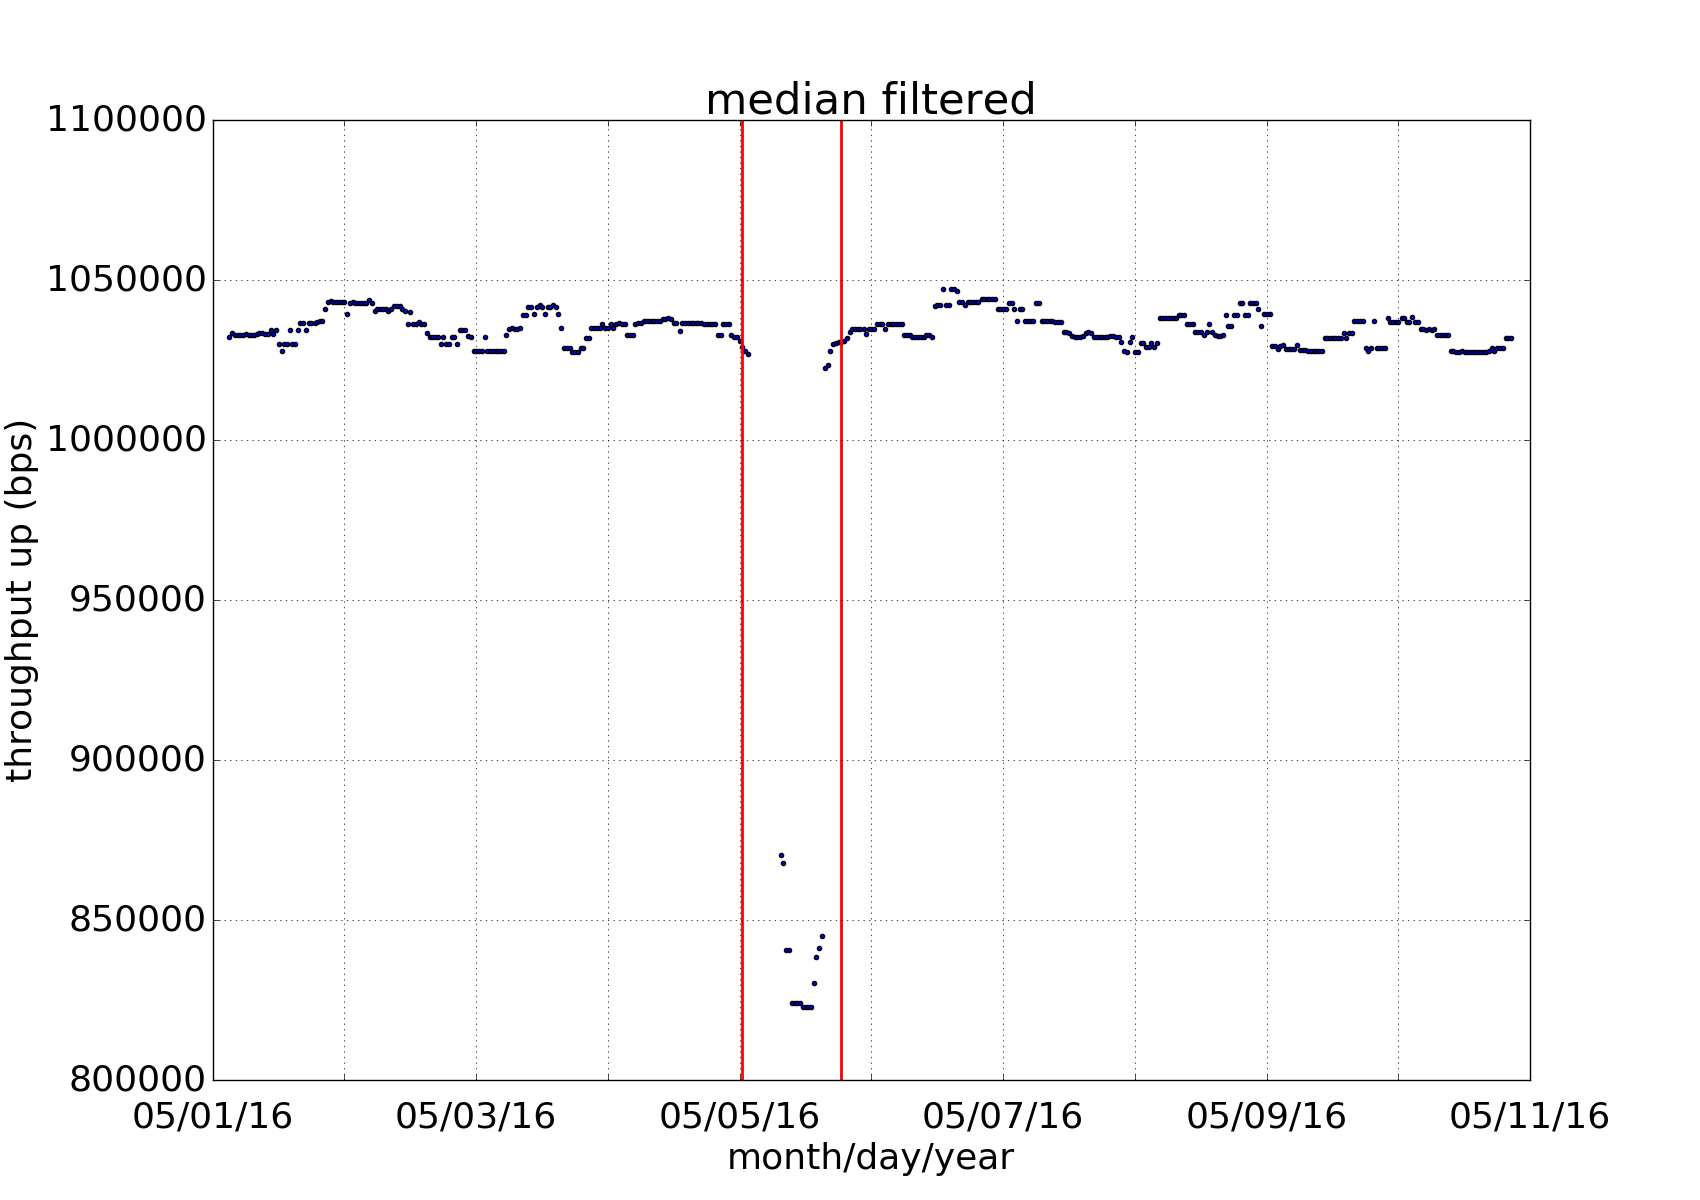
\includegraphics[width=\textwidth]{./figures/results/correct_examples/before_first_hop/serverSDRDTCLDM012_mac64:66:B3:50:06:D4_dtstart2016-05-01_dtend2016-05-11.png}
            \caption{Client 1.}
        \end{subfigure}
        \begin{subfigure}[b]{0.5\textwidth}
            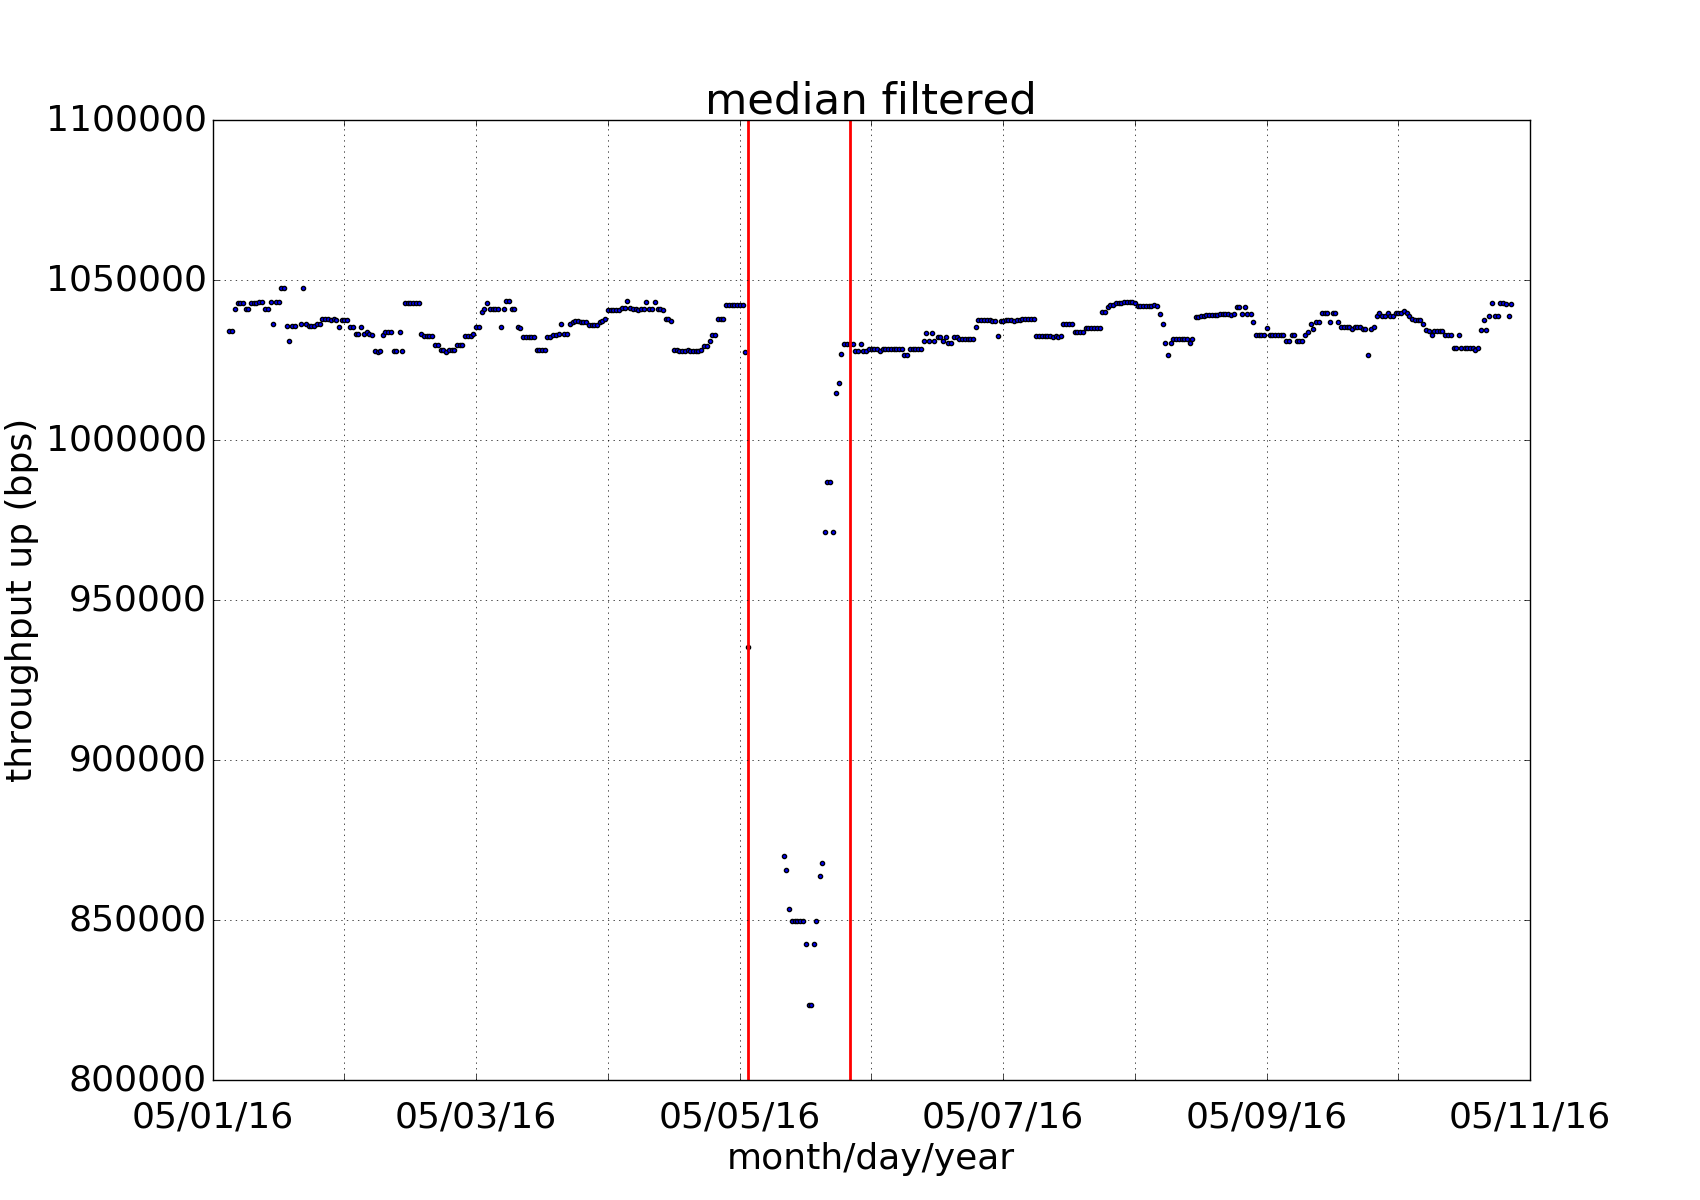
\includegraphics[width=\textwidth]{./figures/results/correct_examples/before_first_hop/serverSDRDTCLDM012_mac64:66:B3:A6:A9:70_dtstart2016-05-01_dtend2016-05-11.png}
            \caption{Client 2.}
        \end{subfigure}%
    }
    \caption{Before first hop.}
\label{fig:before_first_hop}
\end{figure}%

From the 4 clients that belong to this zero indegree user-group, only in those 2
customers the system identified the indicated events.
Therefore, by the estabilished suppositions, they
share a physical equipment before the first hop, that caused these events.

Figure~\ref{fig:zero_indegreee_correlation_client} shows a client with a
specific network event.
Figure~\ref{fig:zero_indegreee_correlation_user_groups_structure} presents an
user-group structure of a server analysis. With exception of the Tier-2
user-group, the groups are defined by a tuple, in which the first field is a
label to the user-group, and the second field represent the fraction of clients
in th euser-group that detected the event illustrated in
Figure~\ref{fig:zero_indegreee_correlation_client}. The gray vertices represent
possible locations resulted from the analysis from a zero indegree vertex to
the server. The blue vertex represent the correlation between these paths
results.

\begin{figure}[H]
    \centering
    \makebox[\textwidth][c]{%
        \begin{subfigure}[b]{0.45\textwidth}
            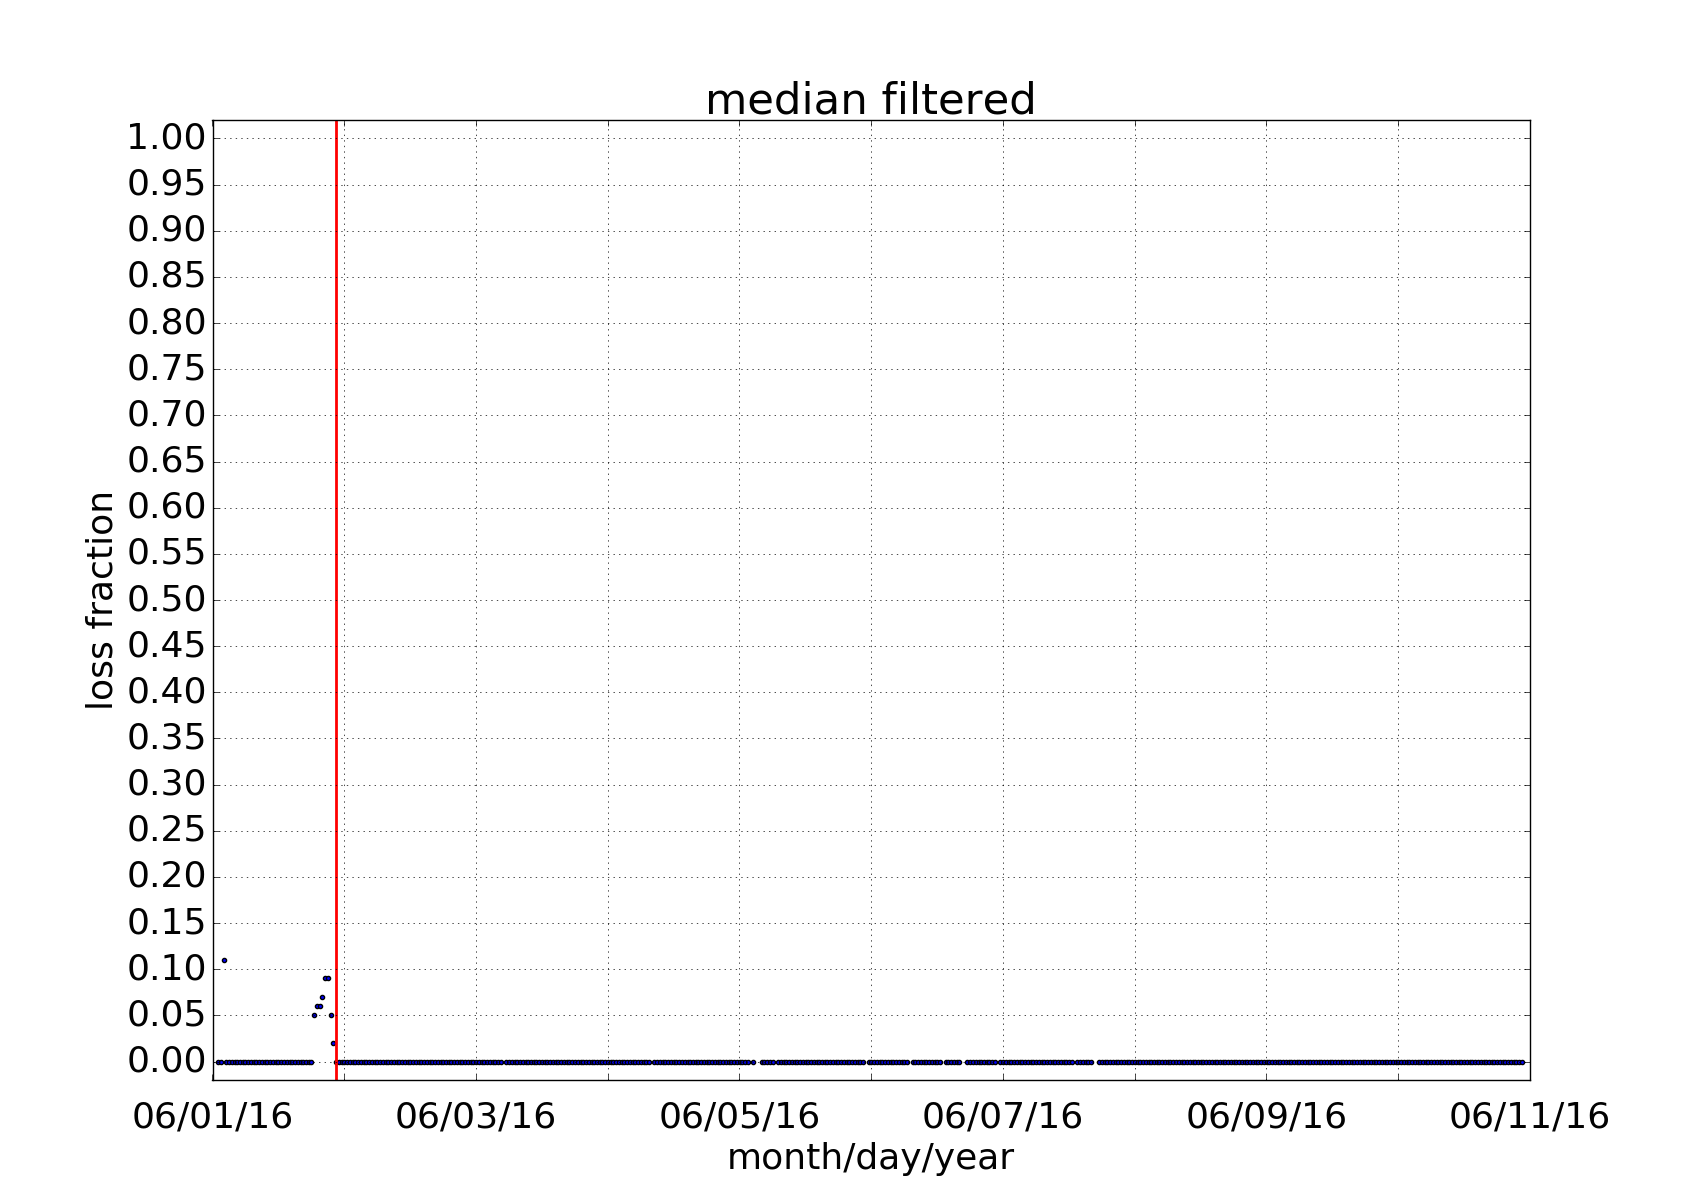
\includegraphics[width=\textwidth]{./figures/results/correct_examples/zero_indegree_correlation/serverSOCDTCPEV01_mac64:66:B3:4F:EA:E2_dtstart2016-06-01_dtend2016-06-11.png}
            \caption{Client 1.}\label{zero_indegree_correlation_client}
        \end{subfigure}
        \begin{subfigure}[b]{0.65\textwidth}
            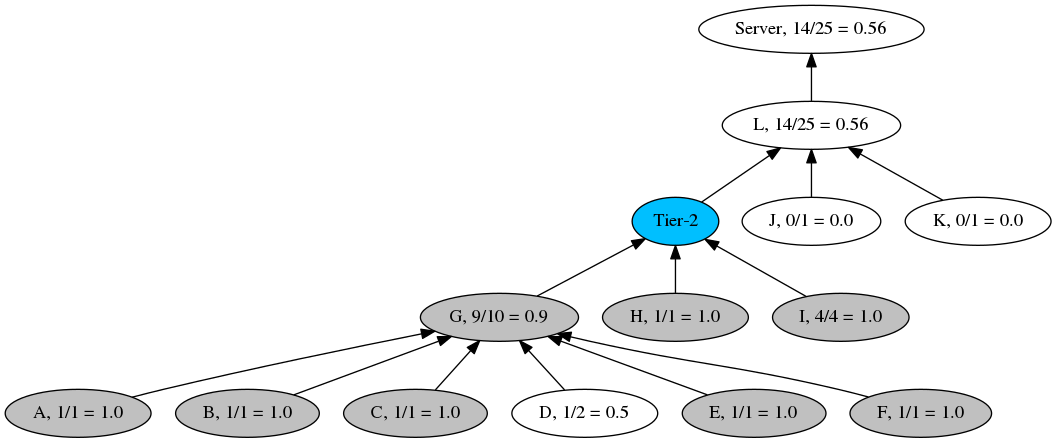
\includegraphics[width=\textwidth]{./figures/results/correct_examples/zero_indegree_correlation/dtstart2016-06-01_dtend2016-06-11_SOCDTCPEV01_traceroute_compress_embratel_graph_anonymized.png}
            \caption{User-groups structure.}\label{zero_indegree_correlation_user_groups_structure}
        \end{subfigure}%
    }
    \caption{Zero indegree vertices results correlation.}
\label{fig:zero_indegreee_correlation}
\end{figure}%

It was visually verified that the same change point pattern of
Figure~\ref{fig:zero_indegreee_correlation_client} is present in all clients
that belong to vertexes A to I. For instance, this event was not correctly
identified in one client of D, however it was visually verified that it was a
wrong classification.

In Figure~\ref{fig:zero_indegreee_without_correlation} it is an example of a
network event in which location was only identified in one zero indegree
user-group.

\begin{figure}[H]
    \centering
    \makebox[\textwidth][c]{%
        \begin{subfigure}[b]{0.45\textwidth}
            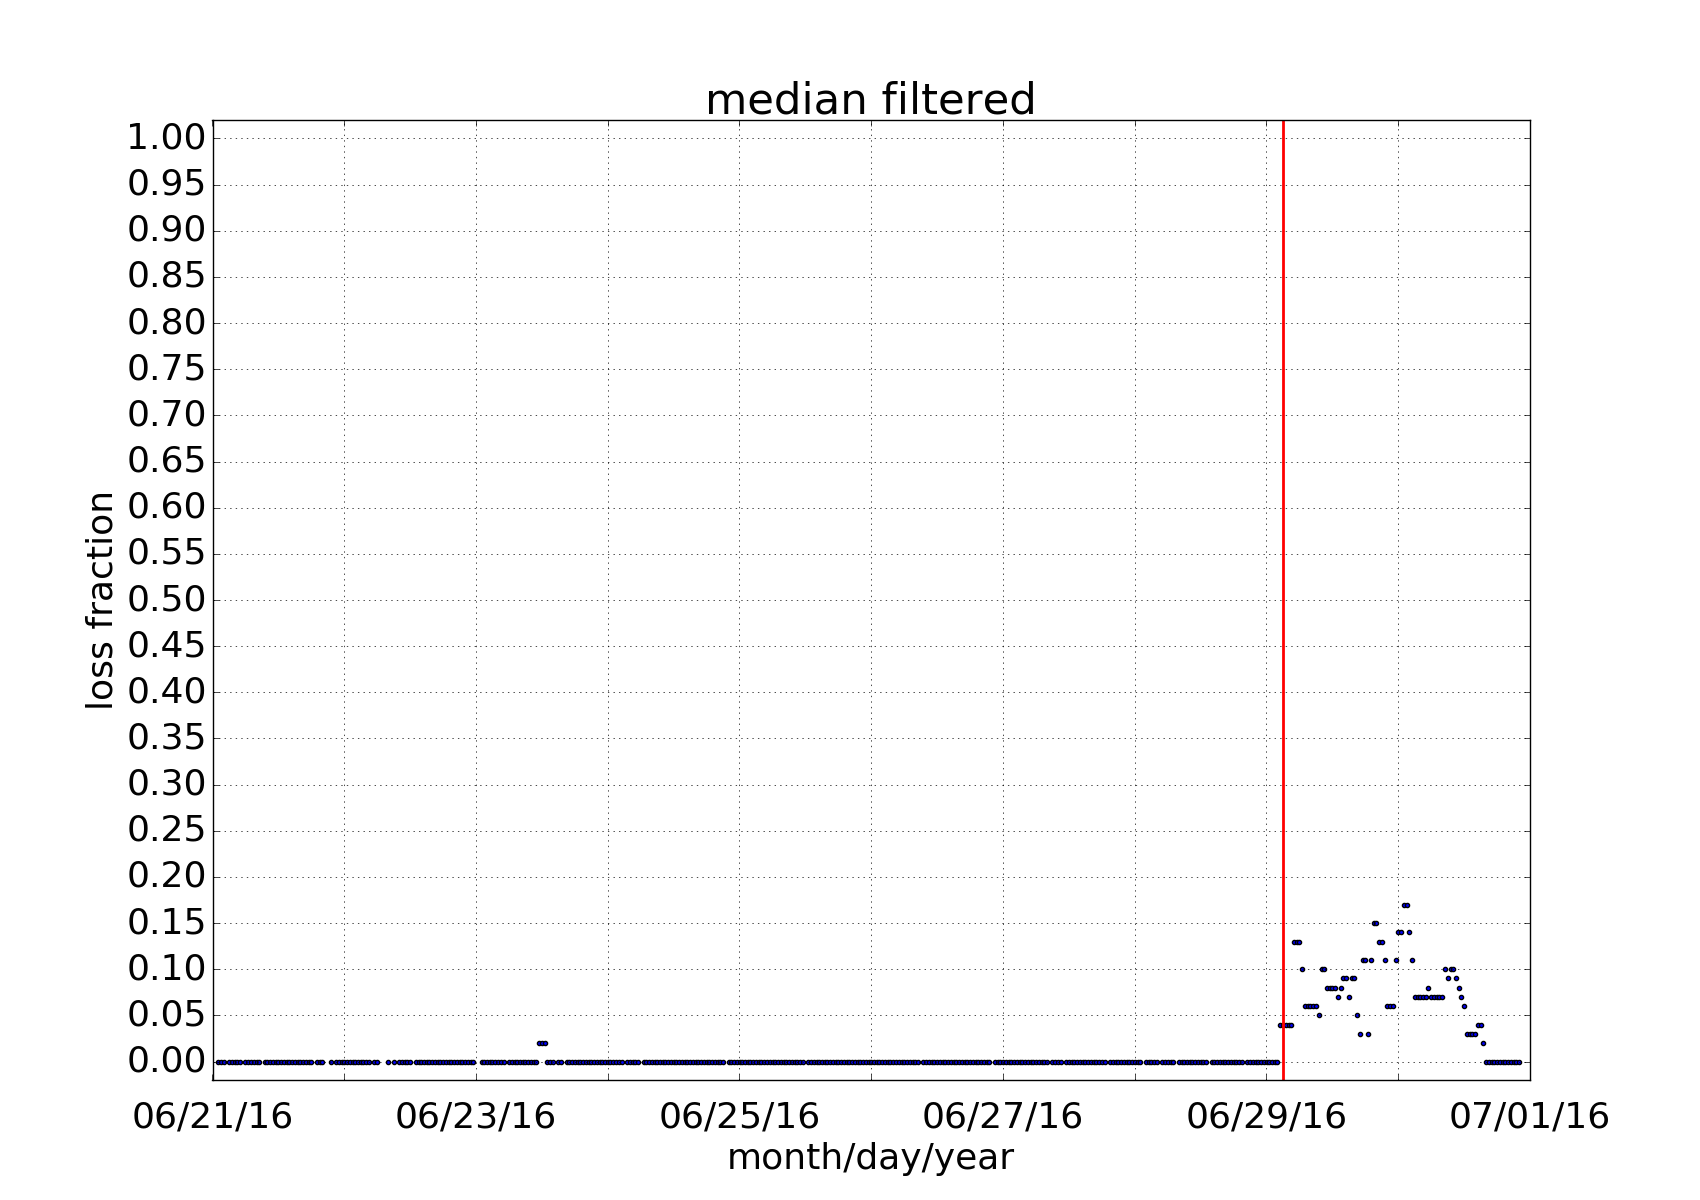
\includegraphics[width=\textwidth]{./figures/results/correct_examples/zero_indegree_single/serverGRSCBCSRV01_mac64:66:B3:50:05:56_dtstart2016-06-21_dtend2016-07-01.png}
            \caption{Client 1.}
        \end{subfigure}
        \begin{subfigure}[b]{0.65\textwidth}
            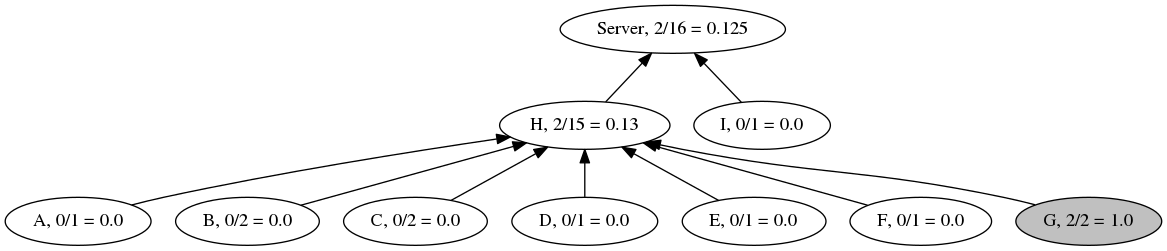
\includegraphics[width=\textwidth]{./figures/results/correct_examples/zero_indegree_single/dtstart2016-06-21_dtend2016-07-01_GRSCBCSRV01_traceroute_compress_embratel_filter_graph_anonymized.png}
            \caption{User-groups structure.}
        \end{subfigure}%
    }
    \caption{Network event in only one zero indegree user-group.}
\label{fig:zero_indegreee_without_correlation}
\end{figure}%

Table~\ref{table:number_of_events} summarizes the number of events considering
the previous three cases types. It weren't detected inconclusive events.

\begin{table}[]
\centering
\begin{tabular}{|c|c|c|c|c|c|c|}
\hline
\multirow{3}{*}{Metric}                & \multicolumn{6}{c|}{Events}                                                                                                                                                                                                                \\ \cline{2-7}
                                       & \multicolumn{2}{c|}{Before first hop} & \multicolumn{2}{c|}{\begin{tabular}[c]{@{}c@{}}Only one zero \\ indegree user-group\end{tabular}} & \multicolumn{2}{c|}{\begin{tabular}[c]{@{}c@{}}Multiple one degree\\ user-groups\end{tabular}} \\ \cline{2-7}
                                       & Improvement         & Failure         & Improvement                                       & Failure                                       & Improvement                                      & Failure                                     \\ \hline
RTT                                    & 688                 & 685             & 789                                               & 809                                           & 43                                               & 38                                          \\ \hline
Round trip loss fraction               & 167                 & 144             & 141                                               & 116                                           & 2                                                & 2                                           \\ \hline
Maximum achievable upstream throughput & 395                 & 358             & 331                                               & 280                                           & 4                                                & 3                                           \\ \hline
\end{tabular}
\caption{Number of events.}
\label{table:number_of_events}
\end{table}

\section{Possible Wrong Outcomes}
\label{sec:possible_wrong_outcomes}

Figure~\ref{fig:time_correlation_unmatch} presents two clients that belong to
the same zero indegree user-group.

\begin{figure}[H]
    \centering
    \makebox[\textwidth][c]{%
        \begin{subfigure}[b]{0.5\textwidth}
            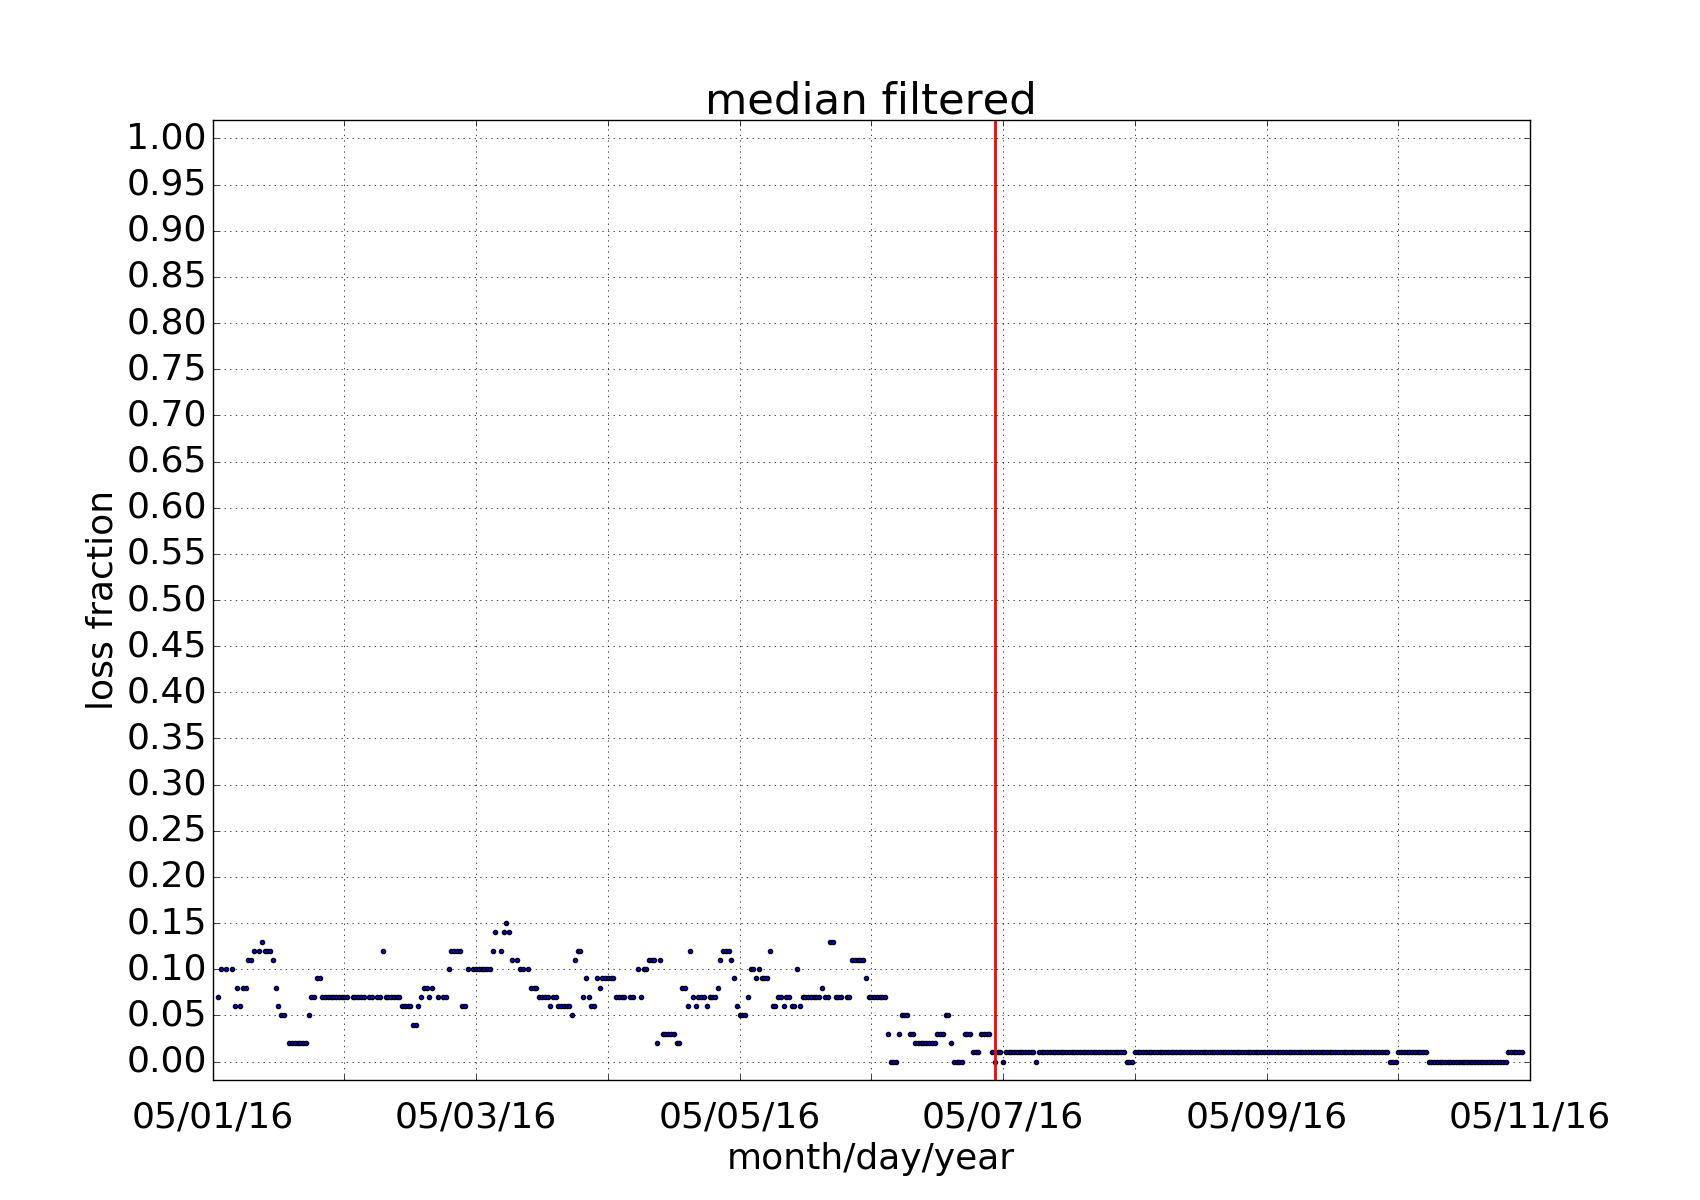
\includegraphics[width=\textwidth]{./figures/results/wrong_examples/time_correlation_example/serverSPOTVTSRV16_mac64:66:B3:A6:AB:80_dtstart2016-05-01_dtend2016-05-11.png}
            \caption{Client 1.}\label{fig:time_correlation_unmatch_client1}
        \end{subfigure}
        \begin{subfigure}[b]{0.5\textwidth}
            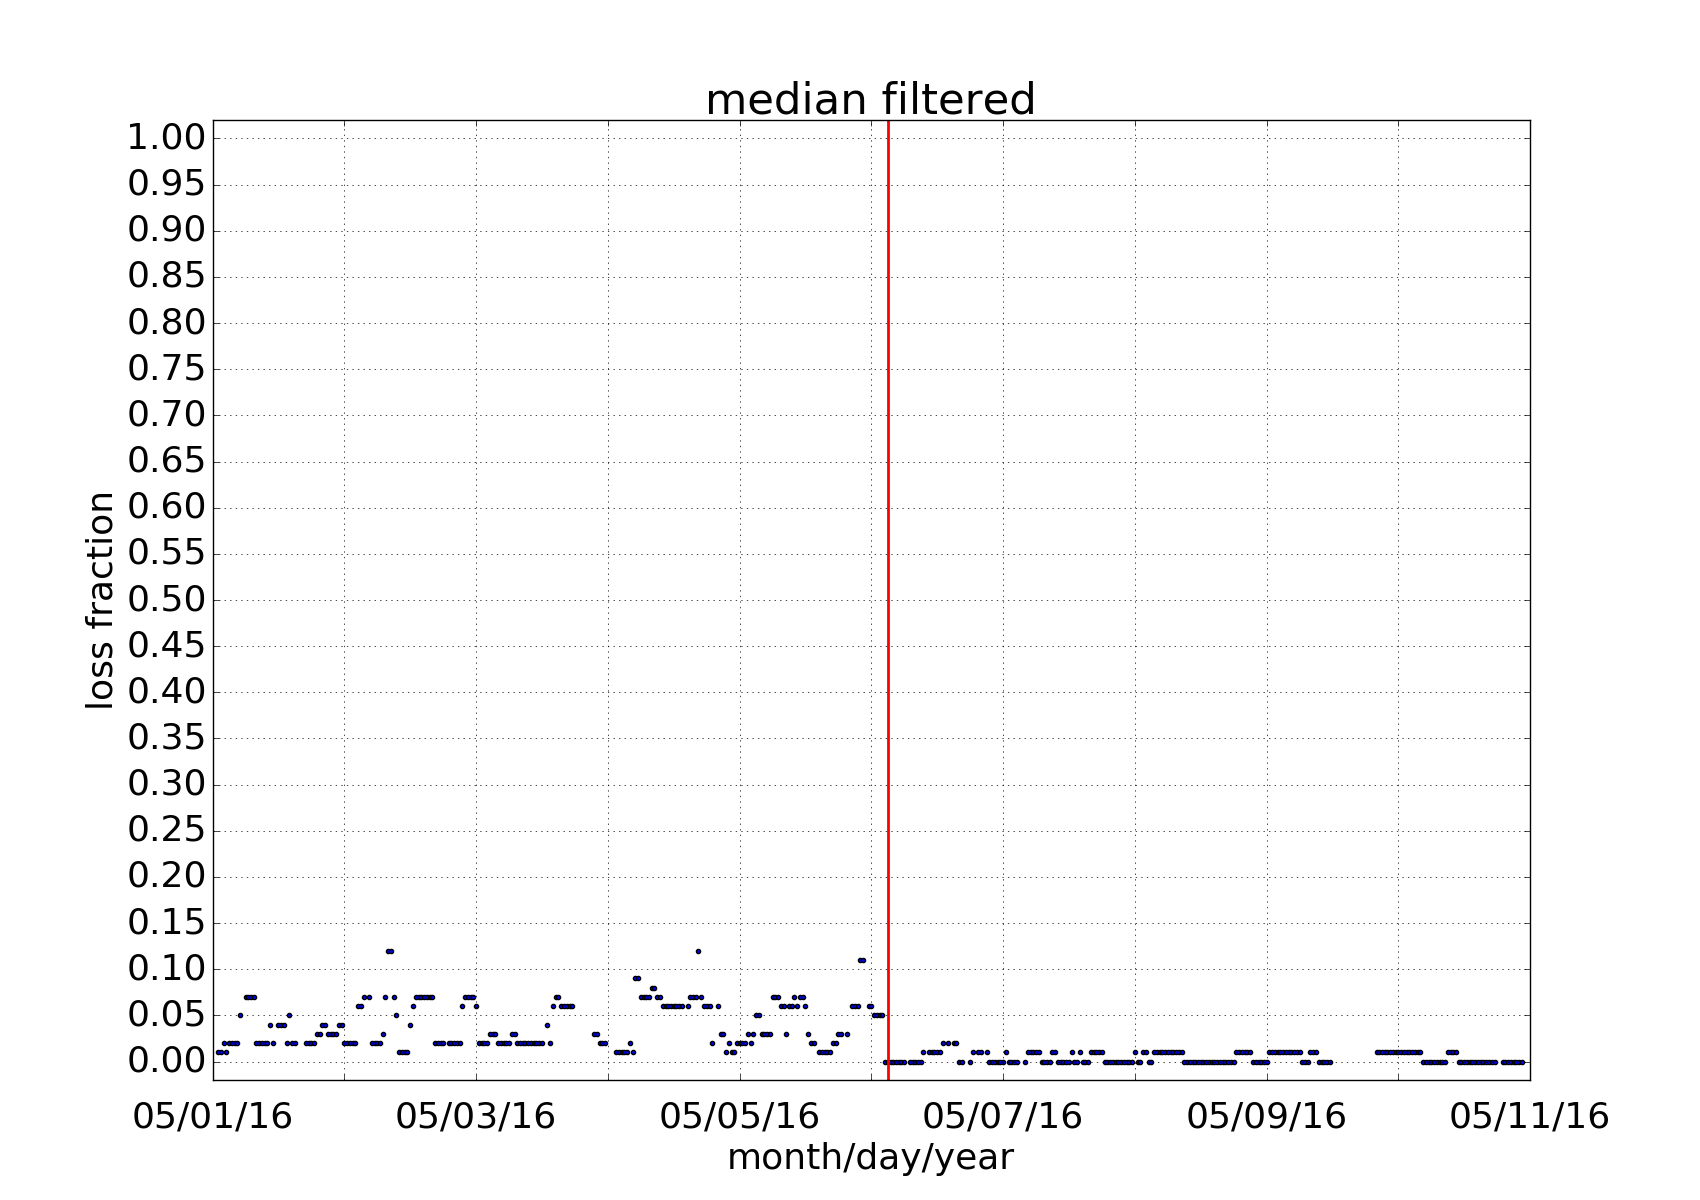
\includegraphics[width=\textwidth]{./figures/results/wrong_examples/time_correlation_example/serverSPOTVTSRV16_mac64:66:B3:A6:AC:40_dtstart2016-05-01_dtend2016-05-11.png}
            \caption{Client 2.}\label{fig:time_correlation_unmatch_client2}
        \end{subfigure}%
    }
    \caption{Time correlation unmatch.}
\label{fig:time_correlation_unmatch}
\end{figure}%

Both client, visually have the similar change point patterns. However, due to
the change point detection algorithm and the time correlation procedures, the
system detected that these clients don't share the same networ event. From the
same zero indegree user-group of those clients, the system detected a network
event in all 17 customers. Correlating the events times, it was defined to two
network events, one more close to client 1 and other to client 2. However,
visually seems that only one event occurred. Then instead of detecting all the
zeroindegree user-group as a possible cause, it were detected two proper subset
of clients with cause before the first hop.

Figure~\ref{fig:untraceable_location} shows two change patterns.

\begin{figure}[H]
    \centering
    \makebox[\textwidth][c]{%
        \begin{subfigure}[b]{0.5\textwidth}
            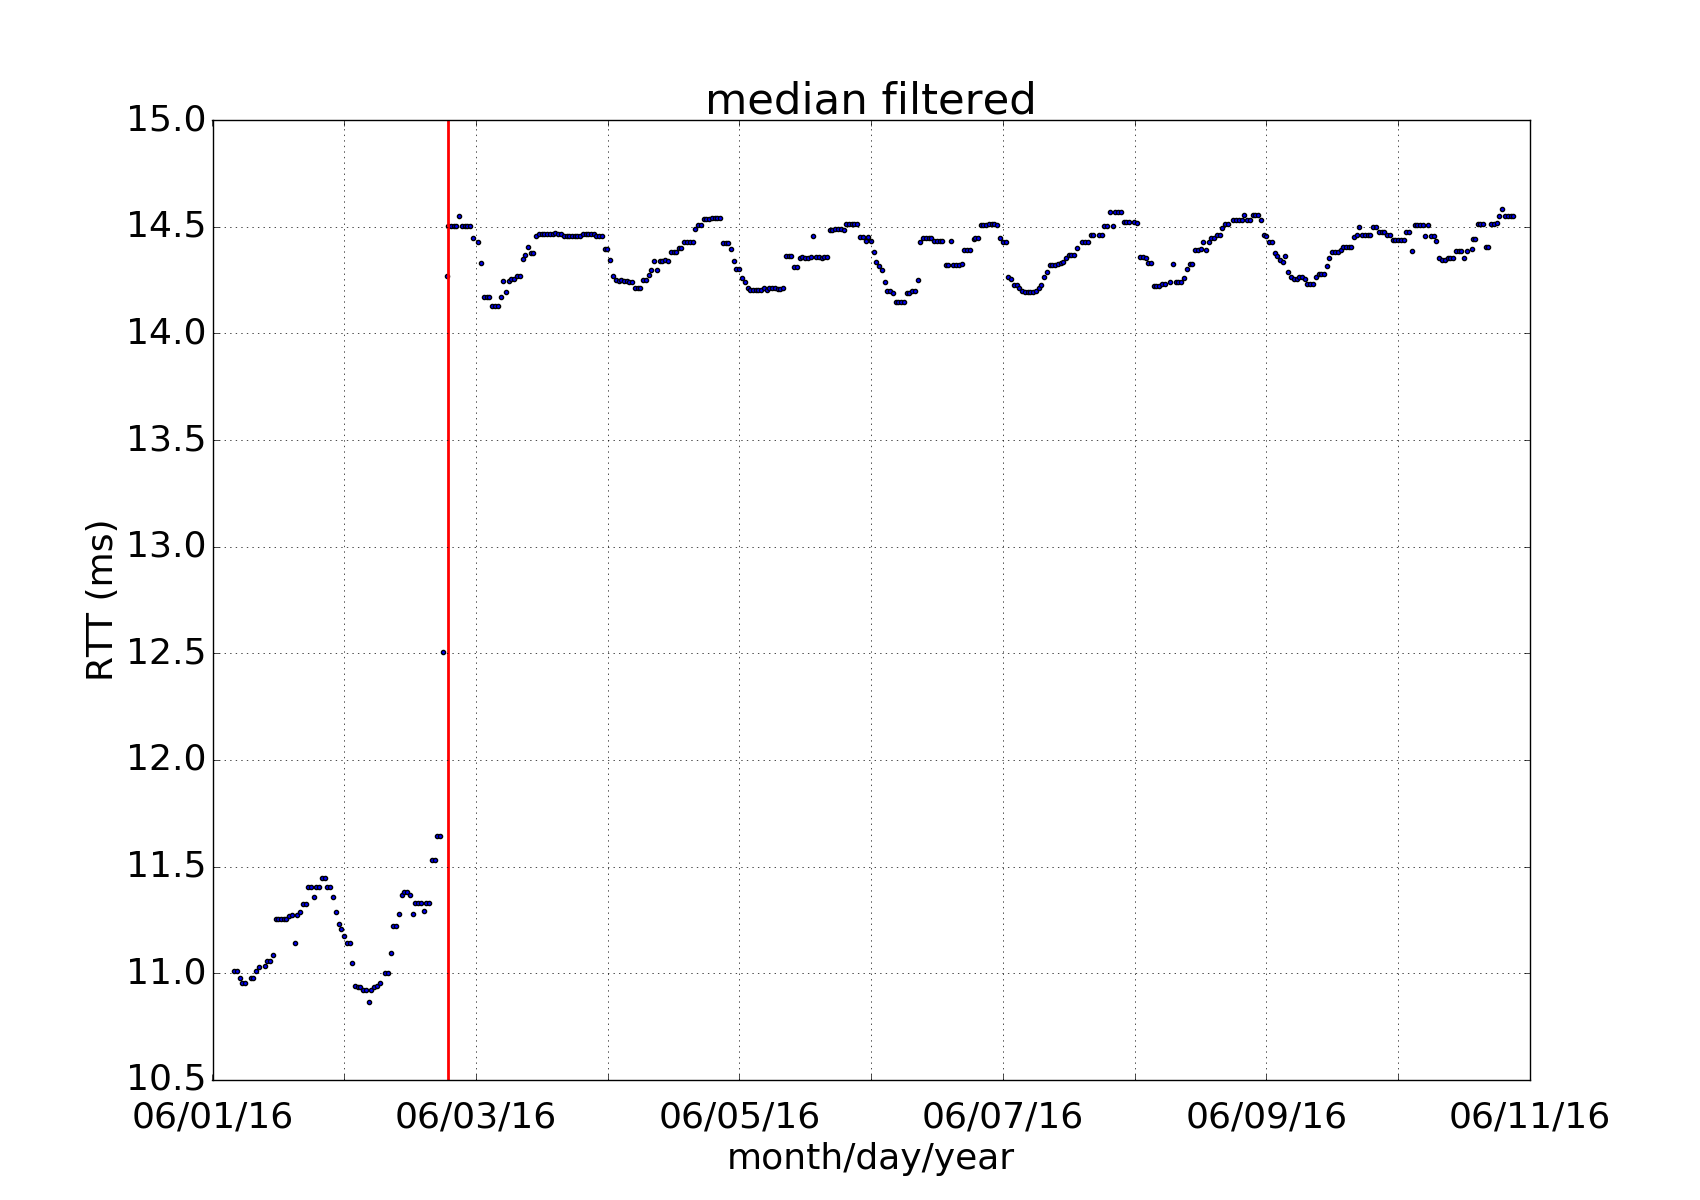
\includegraphics[width=\textwidth]{./figures/results/wrong_examples/untraceable_example/serverBHZDTCLDM062_mac64:66:B3:50:00:68_dtstart2016-06-01_dtend2016-06-11.png}
            \caption{Client 1.}\label{fig:untraceable_location_client_1}
        \end{subfigure}
        \begin{subfigure}[b]{0.5\textwidth}
            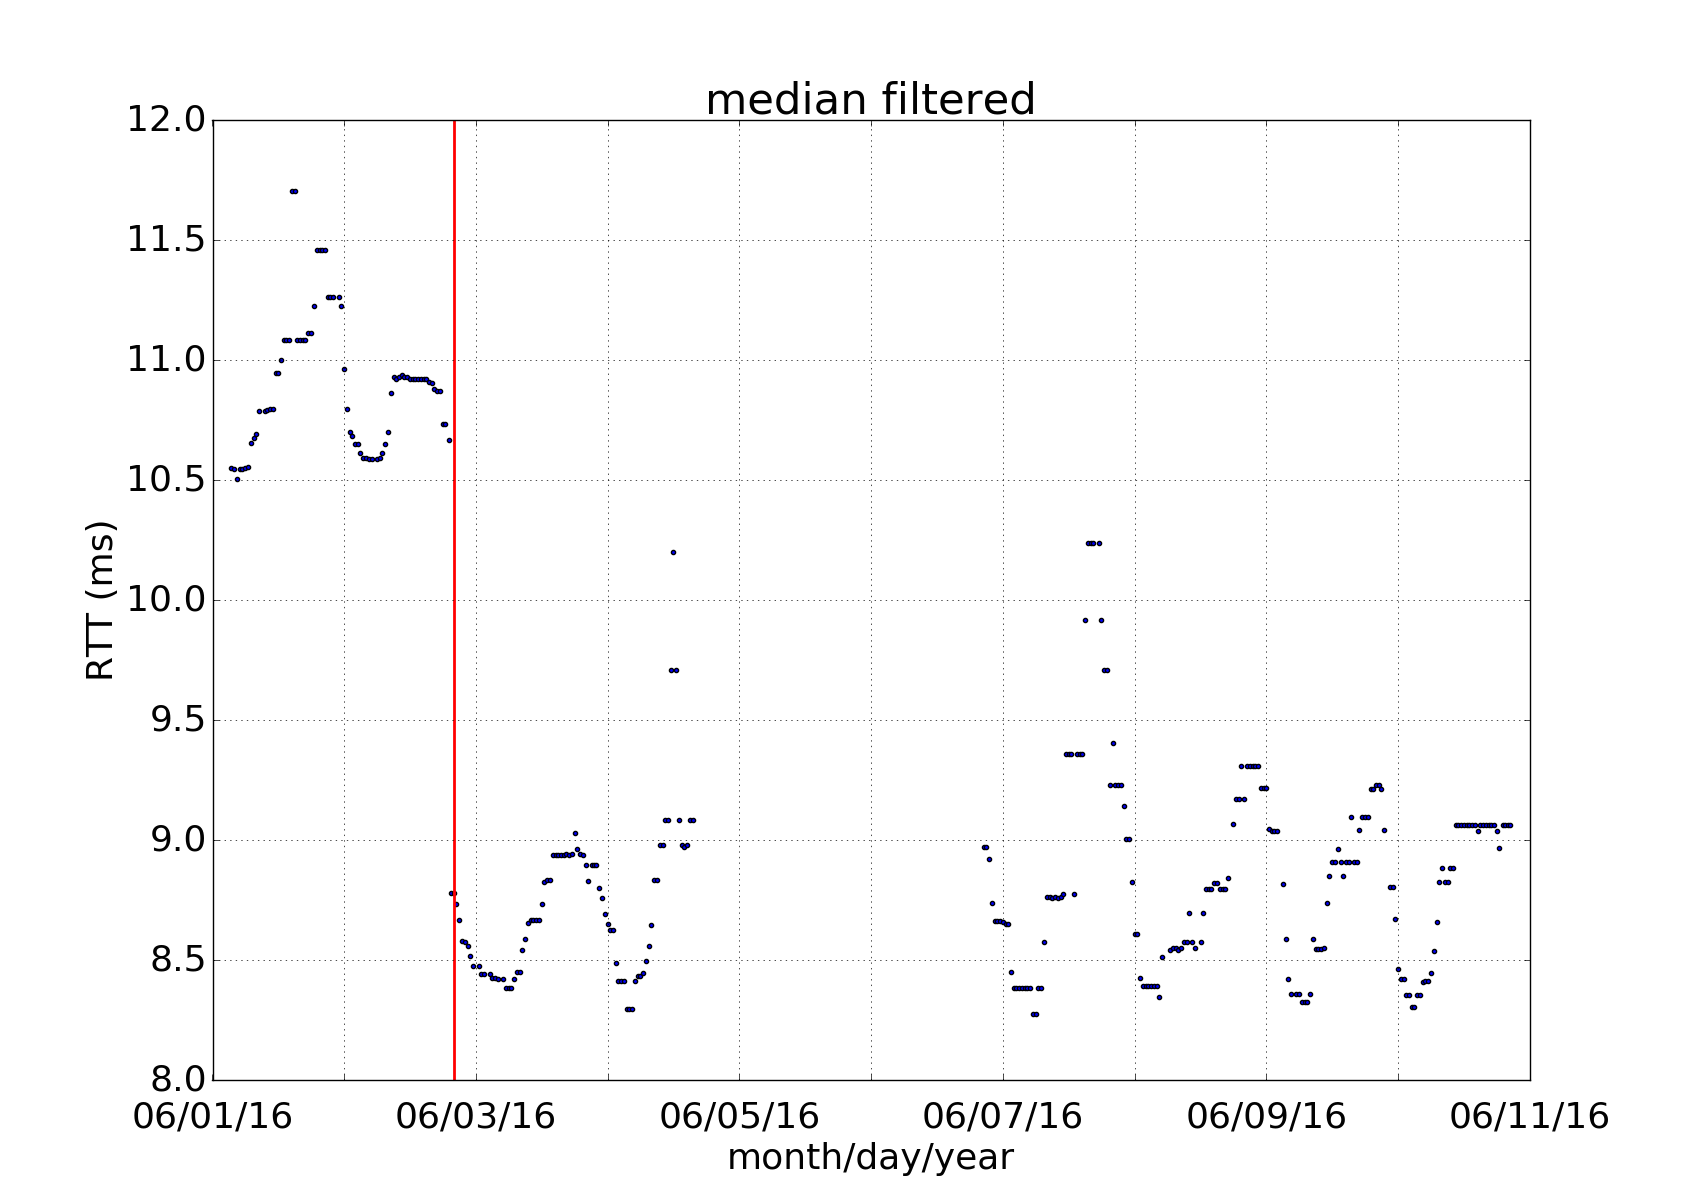
\includegraphics[width=\textwidth]{./figures/results/wrong_examples/untraceable_example/serverBHZDTCLDM062_mac64:66:B3:50:00:B6_dtstart2016-06-01_dtend2016-06-11.png}
            \caption{Client 2.}\label{fig:untraceable_location_client_2}
        \end{subfigure}%
    }
    \caption{Untraceable location.}
\label{fig:untraceable_location}
\end{figure}%

Both clients belong to the same zero indegree vertex,
and in this case the traffic of the clients doesn't go to the Tier-2 ISP.
It was verified that several clients that doesn't share any equipments that
appear in the traceroute, and measure to different servers, and are located in
different Brazilian UFs present a change pattern at the same time in the RTT
metric. Additionaly, in some clients there is an Improvement, while in other
there is a failure. DUring the 5 months, it were manually detected three cases
like that, and was only detected in the RTT time series, it were not found this
pattern in the other metrics. Possibly this changes are correlated, since
this would be a unlikely coincidence. However, since the changes occurred in
different clients in different network regions, the cause of this event should
be a global network change. For instance could be a centralized parametere
change deployed by the ISP that are propagated to access home routers
simultaneously. Also it could be a change in the measurement software. The
latter case was verified and was not the cause. However this work doesn't
access to data to check this suppositions. Also it intriguing that some clients
perceive a failure while others an improvement. This kind of changes impact
negatively the system's output, since this kind of event was not considerated
by the suppositions. From Table~\ref{table:number_of_events} a considerable
fraction of the RTT detected events are due to this type of situation.

In some cases, it where manually analysed the RTT per hop between the client to
the server. It was noted that these data can have different patterns in
relation to the used end-to-end RTT. First, the measurement methodologies are
different. Second, as an example, the RTT associated with hop $i$ can ben
constantly and siginficantly bigger then the RTT associated with a hop $j$,
where $j > i$. This can be explained by the fact that some routers prioritizes,
or be optimized to,
forwarding instead of answering ping packets. Therefore, the analysis of this
data was not automally done. For instance, Figure~\ref{fig:rtt_per_hop_client_1}
represents the RTT per hop of the client of
Figure~\ref{fig:untraceable_location_client_1}.
Figure~\ref{fig:rtt_per_hop_client_2} is analogous, however, related to client
of FIgure~\ref{fig:untraceable_location_client_2}.

\section{Final Remarks}

It was detected that several events related to the maximum achievable upstream
throughput consist of a significant mean increase perceived by a single client,
as it is exemplified in Figure~\ref{fig:throughput_up_increase}.
Possibly this kind of event is related to a change in the contracted bandwidth
by the customer.

It was detected that several events detected by only a single zero indegree
user-group were only detected by a single client. For instance,
Figure~\ref{fig:number_of_clients_per_zero_indegree_vertex} is the
histogram of the number of clients per zero indegree vertex.

There are some cases that output possible location are defined by more than one
consecutive vertex that don't represent the Tier-2 ISP. In general this is
caused by the measurement software placement sparsity, as is exemplified in
FIgure~\ref{fig:clients_sparsity}.

It can be noticed that, since the two gray vertexes have the same end-users, it
is not possible to distinguish where the problem can be located, and also
cannot be discarded if the problem is before the first hop.
